\section{Results and Discussions}\label{sec:results}
\subsection{Clustering phase diagrams}\label{sec:res:ct1}
\Cref{fig:result2_synthetic_mds} depicts a two-dimensional representation obtained using MDS with each point corresponding to a phase diagram in the model data set. 
The points are color-coded based on their spectral clustering labels (with a total of five clusters).
In \Cref{fig:result2_synthetic_clusters} we show the representative phase diagrams for each cluster. 
We observe that clusters in~\Cref{fig:synthdata} have distinct features: phase diagrams without any three phase regions (cluster 0); dominant in three phase region (cluster 1); all compositions belonging to three phase (cluster 2); mix of two and three phase regions (cluster 3,4) that differ in the direction of the phase boundary.
It is difficult to determine a way to obtain true clusters: We do more of a context-driven clustering where the hamming distance and number of clusters justify the true/real clusters (See section 5.3 in \cite{TrueClusters}).
In~\Cref{fig:synth_designspace}, we depict the \(\chi\) space sampling as points with \(\chi_{12},\chi_{13}, \chi_{23}\) as coordinate axes. 
The points are then colored based on the clustering label shown in \Cref{fig:result2_synthetic_mds}.
One can observe that the clusters show a radially evolving arrangement, which can be clearly seen in the two-dimensional projection of the design space shown in~\Cref{fig:synth_designspace_2D}.

\begin{figure}[h]\label{fig:synthdata}
    \centering
    \begin{subfigure}[b]{0.48\textwidth}
        \centering
        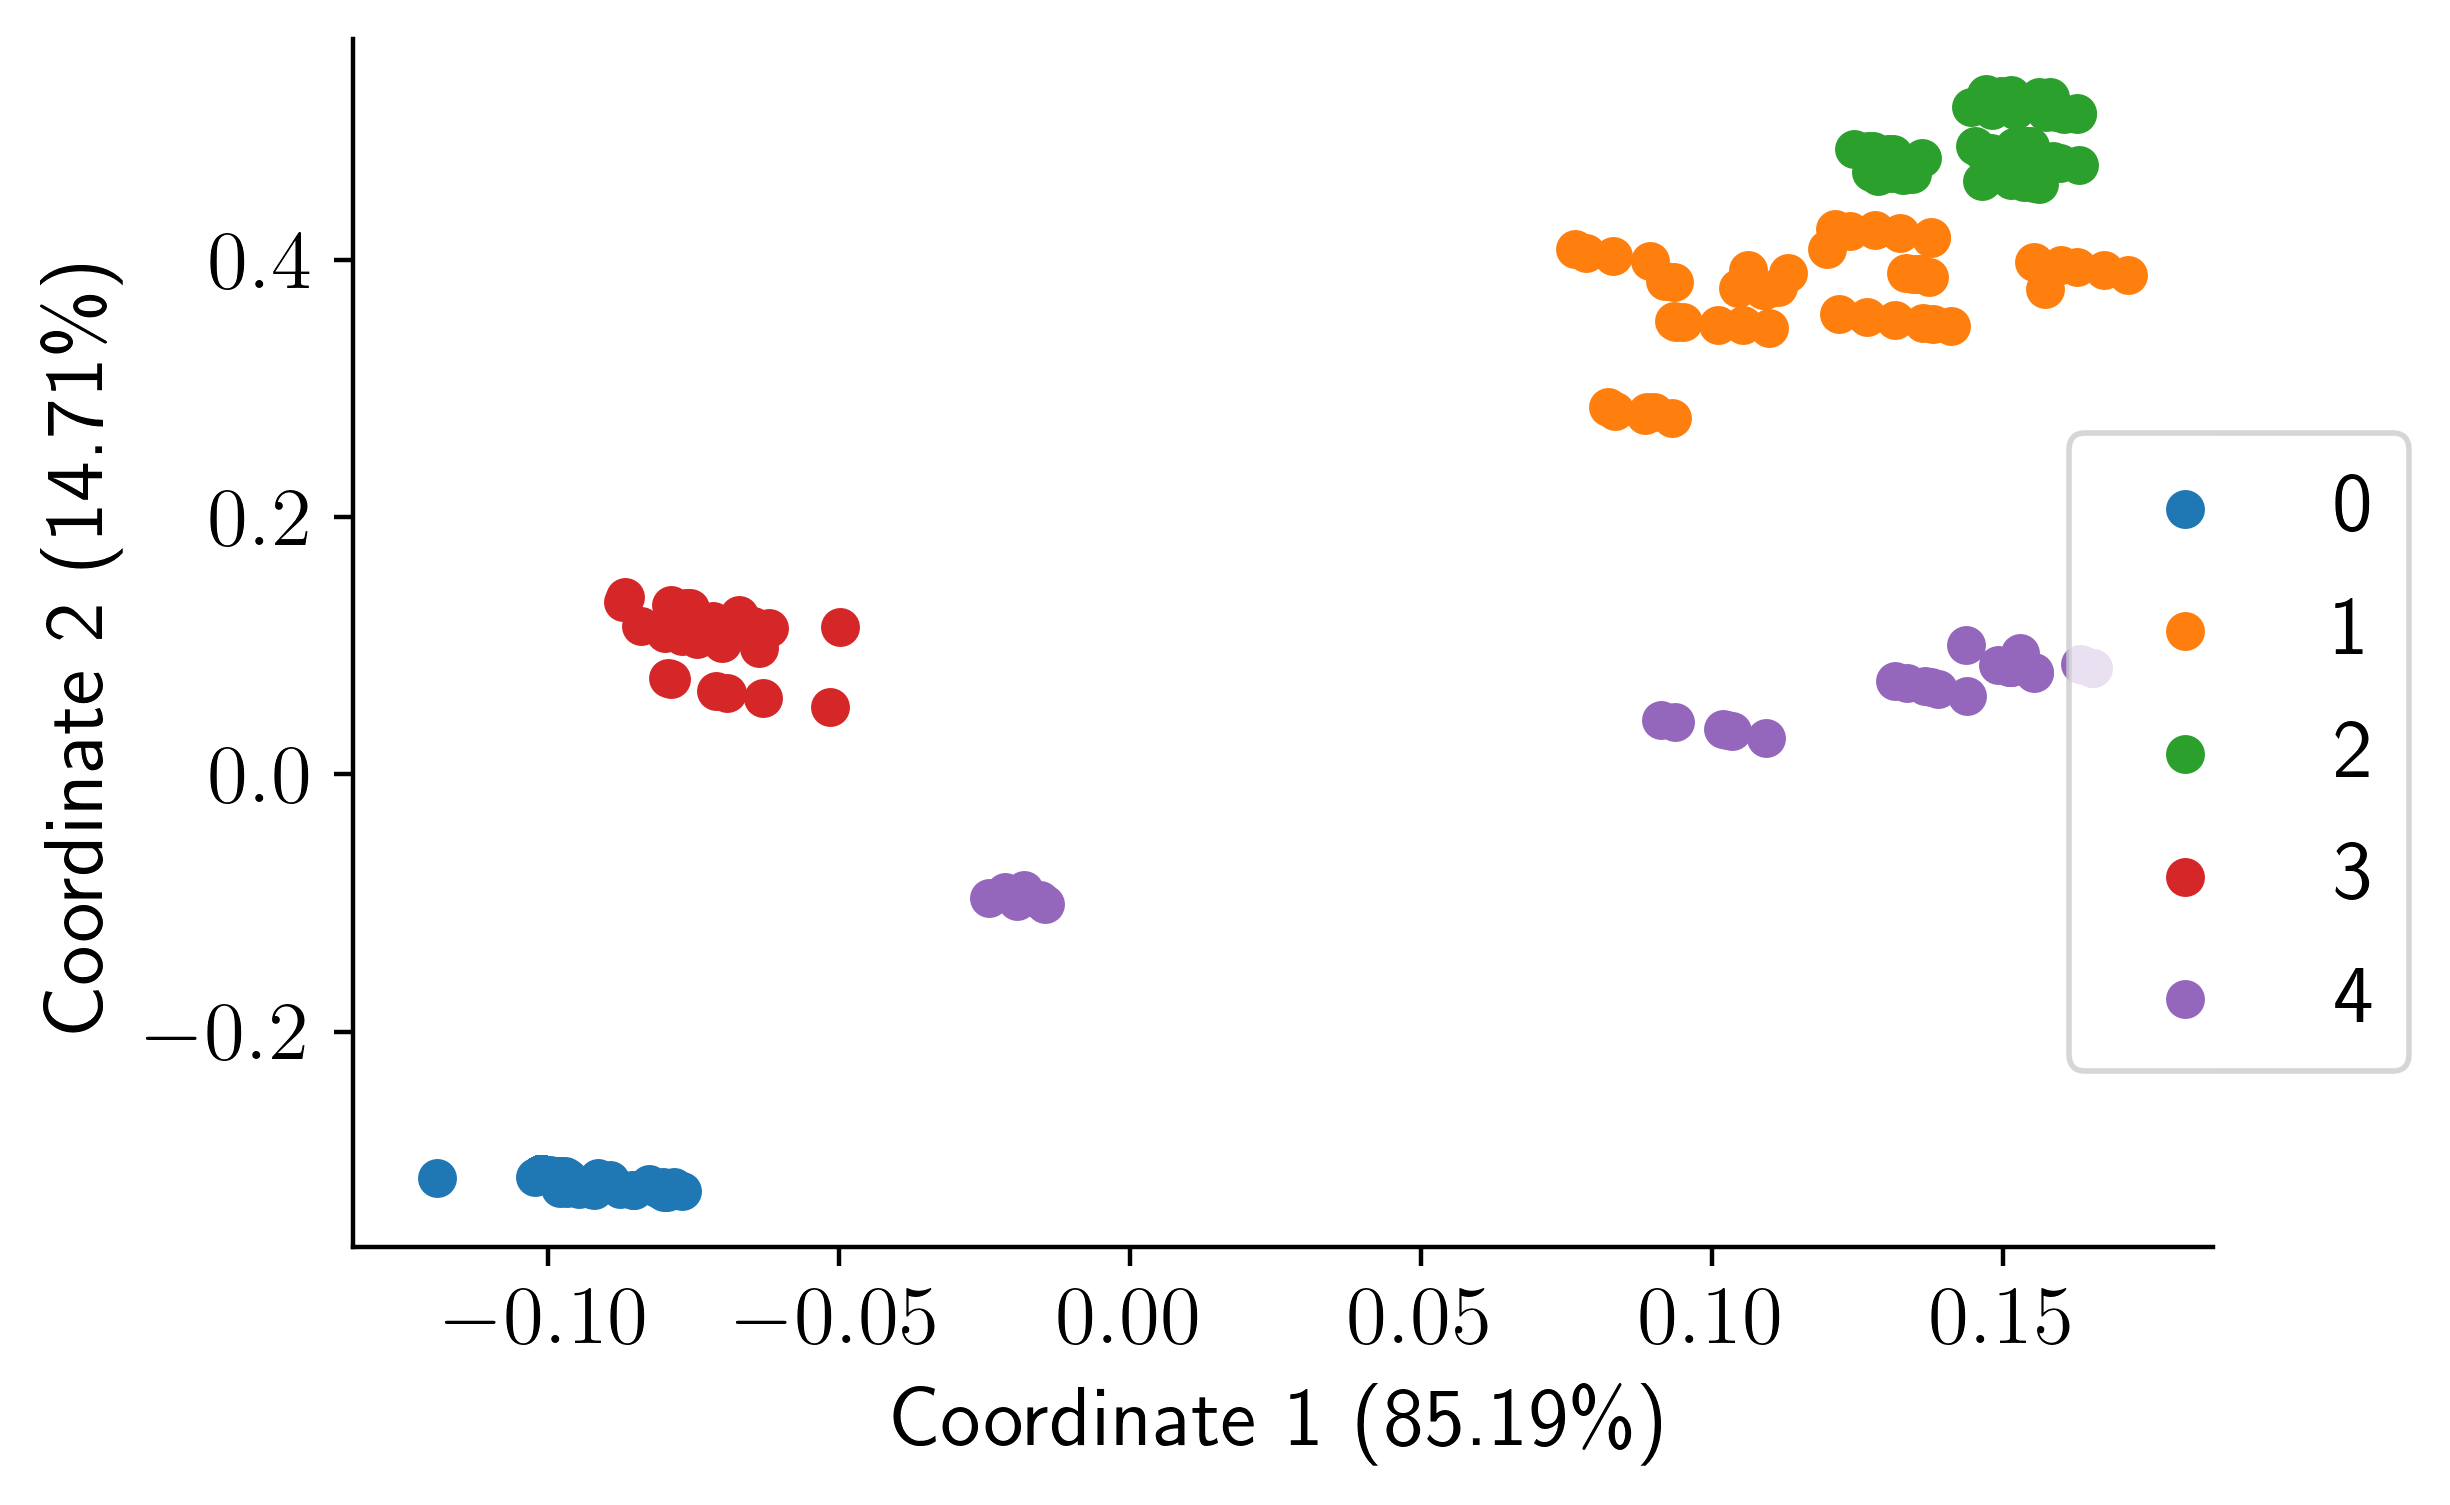
\includegraphics[width=\textwidth]{Chapter-4/figures/result2/result2_Synthetic_MDS.png}
        \label{fig:result2_synthetic_mds}
    \end{subfigure}
    \hfill
    \begin{subfigure}[b]{0.48\textwidth}
        \centering
        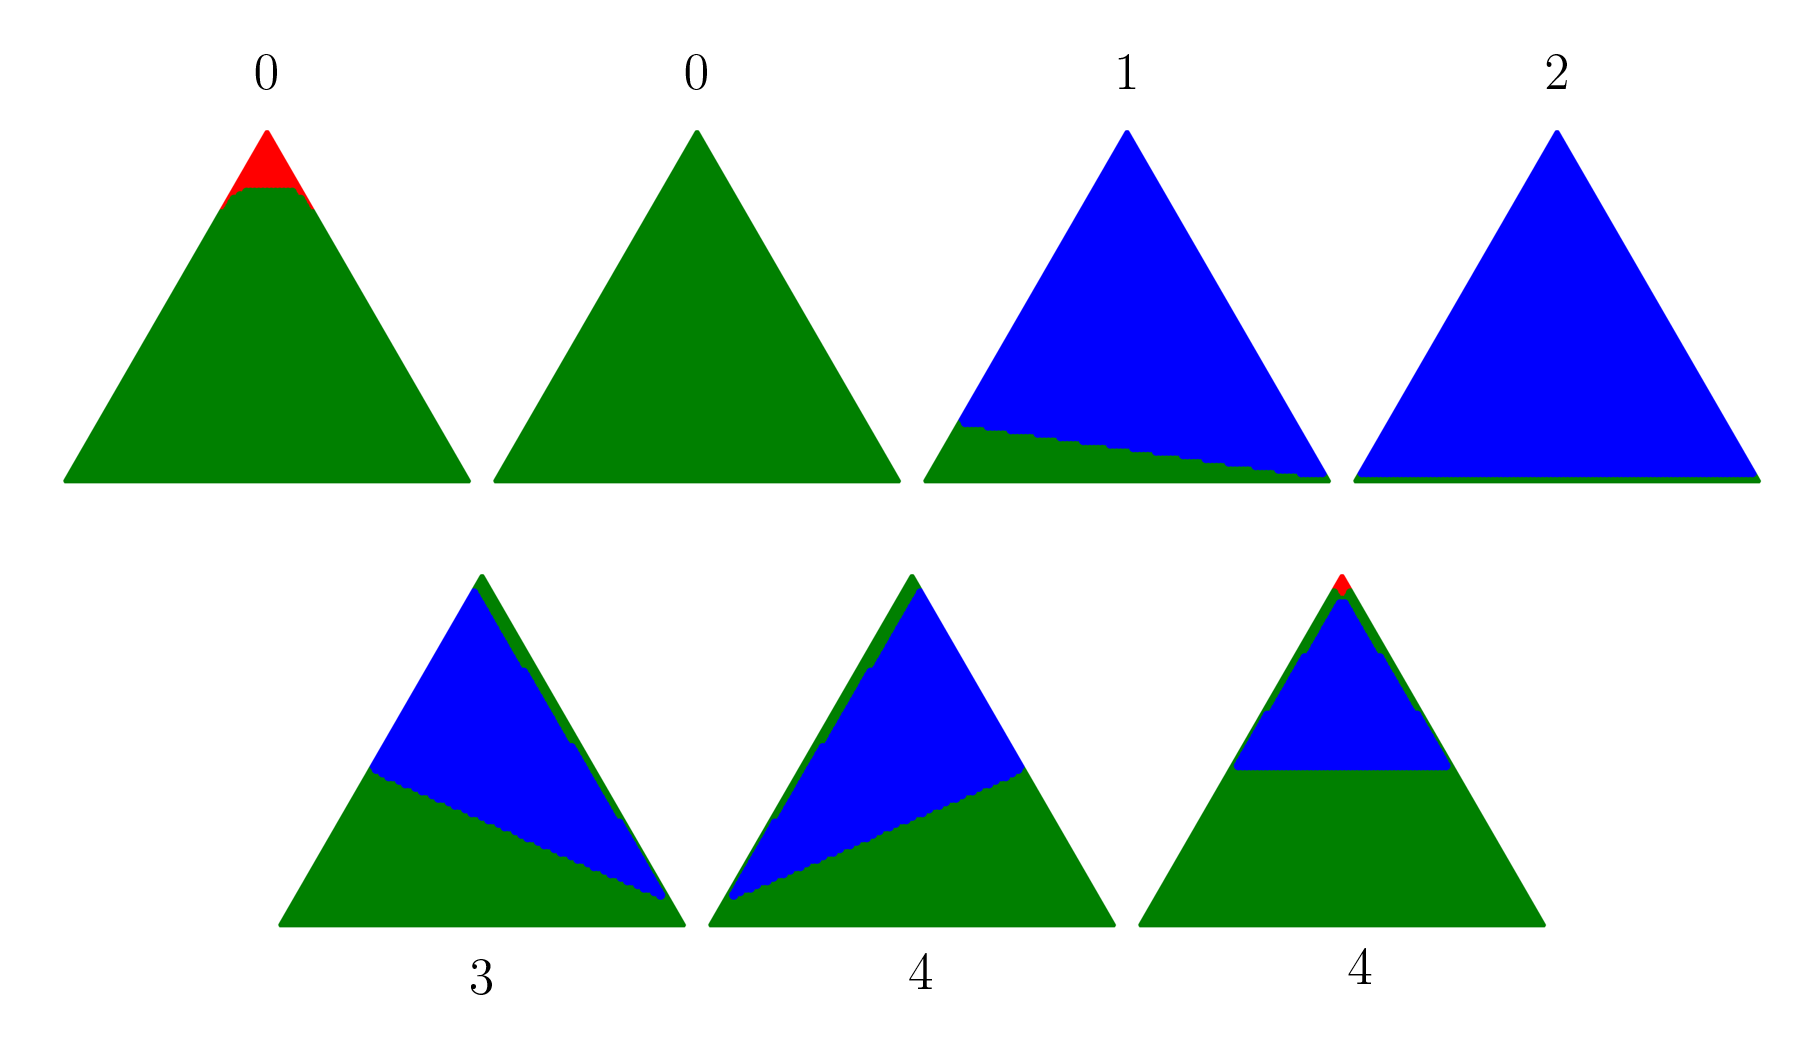
\includegraphics[width=\textwidth]{Chapter-4/figures/result2/result2_synthetic_clusters_manual.png}
        \caption{}
        \label{fig:result2_synthetic_clusters}
     \end{subfigure}
    \caption{Application of data analysis pipeline in \Cref{fig:mlpipeline} to mode data set in \Cref{sec:htedata}. (a) The lower dimensional Euclidean representation of the distance metric \(M\) for the space of 245 phase diagrams obtained for dataset presented in~\Cref{sec:htedata} using MDS. The color-code corresponds to the spectral clustering label. (b) Representative phase diagrams of clusters obtained from spectral clustering of metric \(M\). See text above for the discussion.}
\end{figure}

\begin{figure}[h]
    \centering  
    \begin{subfigure}[b]{0.4\textwidth}
        \centering
        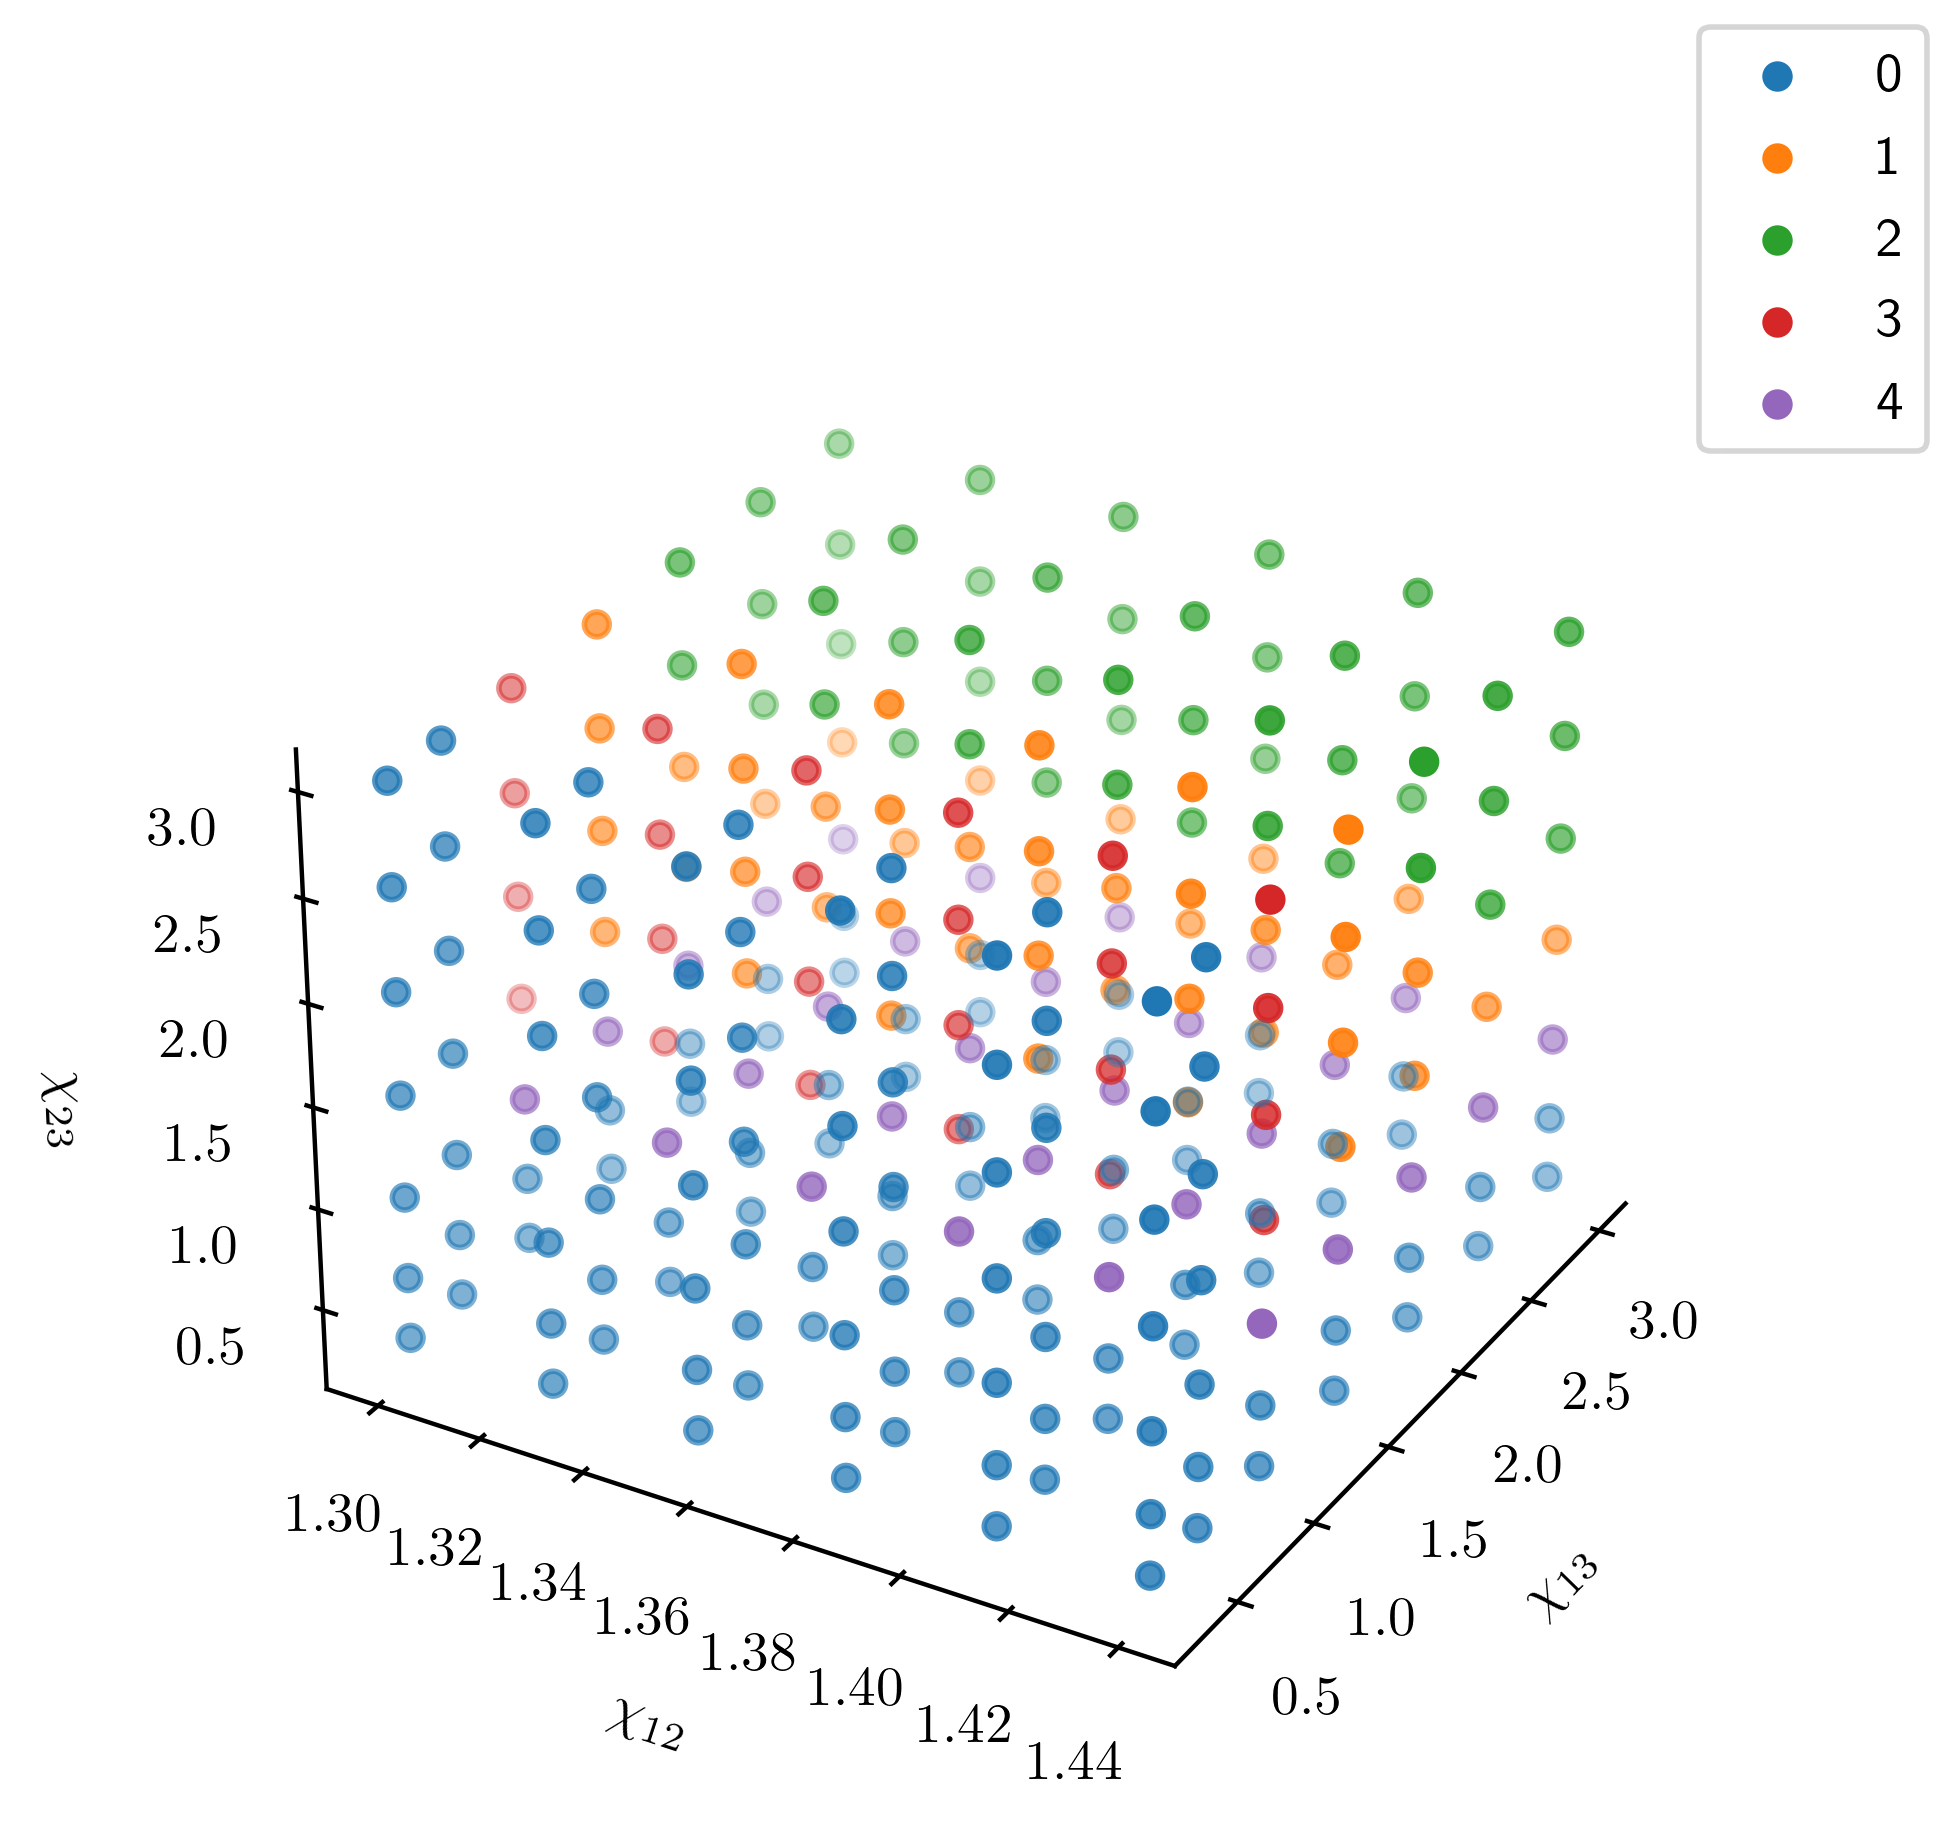
\includegraphics[width=\textwidth]{Chapter-4/figures/result2/result2_Synthetic_DesignSpace.png}
        \caption{}
        \label{fig:synth_designspace_3D}
    \end{subfigure}
    \hfill
    \begin{subfigure}[b]{0.4\textwidth}
        \centering
        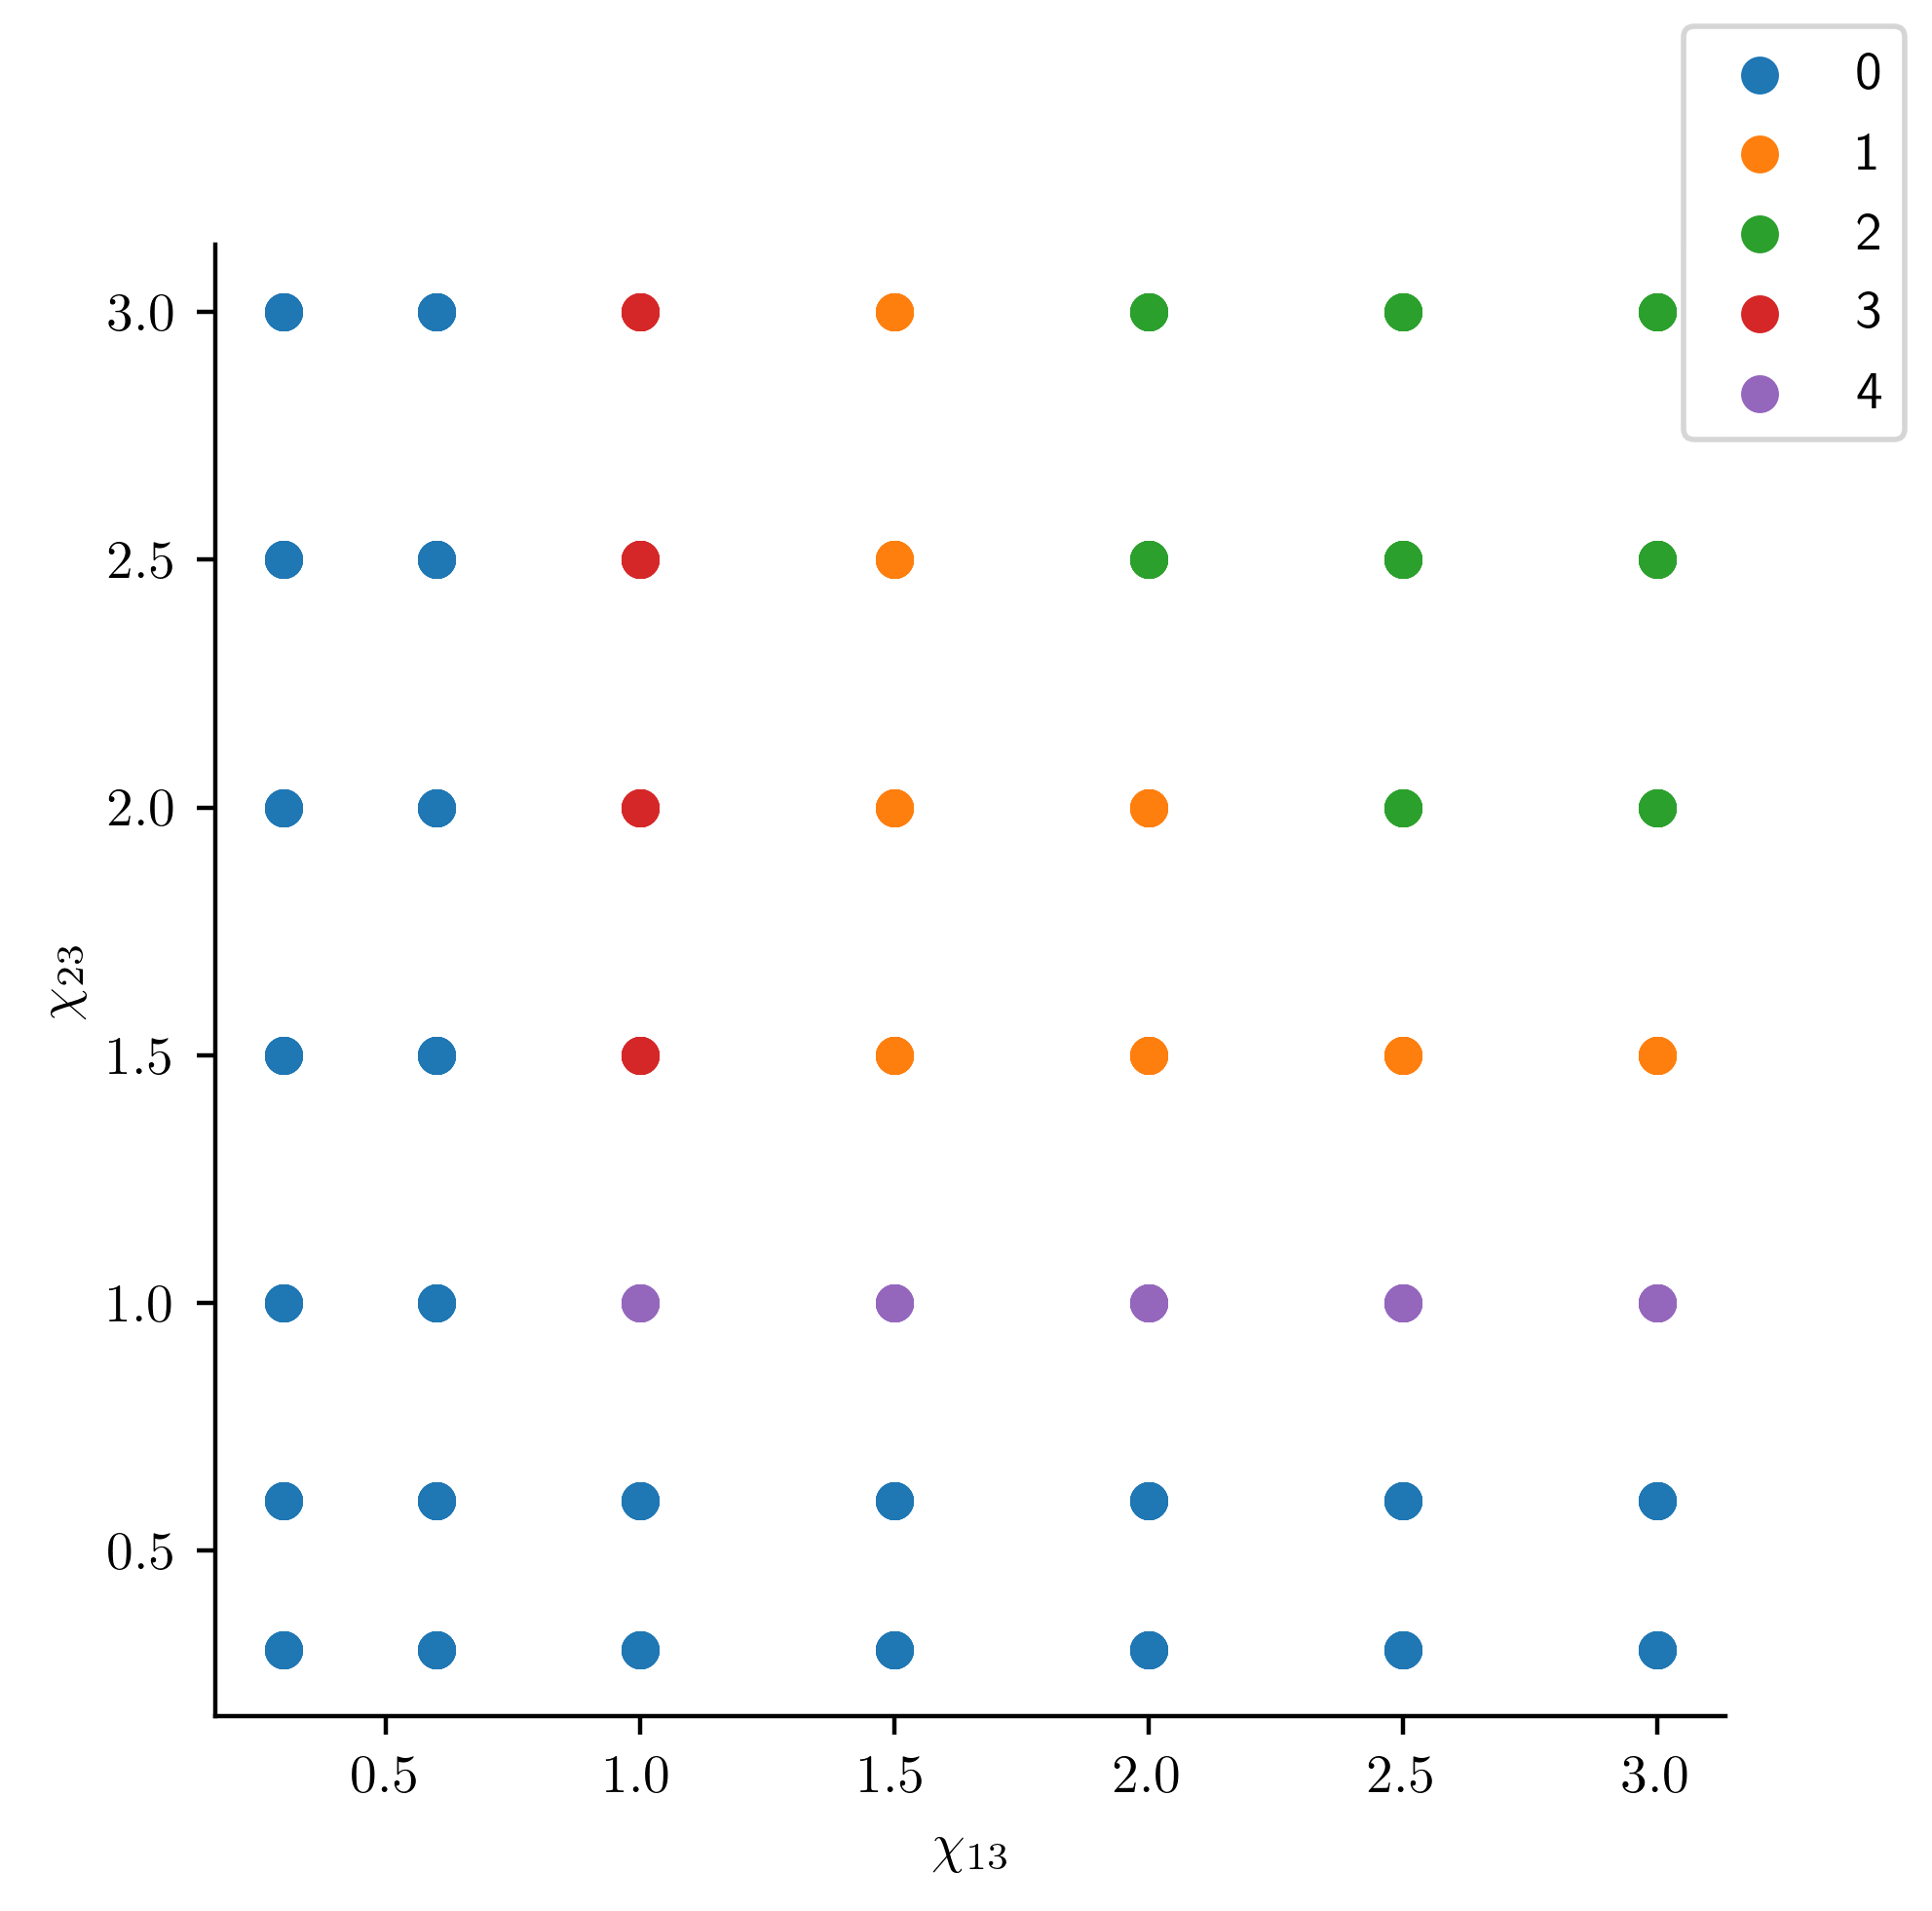
\includegraphics[width=\textwidth]{Chapter-4/figures/result2/result2_Synthetic_DesignSpace_2D.png}
        \caption{}
        \label{fig:synth_designspace_2D}
     \end{subfigure}
    \caption{Design space for model systems data set with points are color-coded with corresponding the cluster index of the phase diagram corresponds. (a) Input sampling space with \(\chi\) values as coordinates.Each point is colored based on their corresponding clustering label. (b) A radial trend in the clusters can be observed when visualizing the clusters on a two-dimensional projection of only \(\chi_{13}, \chi_{23}\).}
    \label{fig:synth_designspace}
\end{figure}
